\documentclass[a4paper]{article}
\usepackage[utf8]{inputenc}
\usepackage[T1]{fontenc}
\usepackage[slovene]{babel}
\usepackage{lmodern}
\usepackage{hyperref}
\usepackage{blindtext}
\usepackage{amssymb}  
\usepackage{listings} %python koda
\usepackage{graphicx}

\begin{document}

\begin{titlepage}
\center
\textsc{\LARGE Univerza v Ljubljani}\\[0.5cm]
\textsc{\Large Fakulteta za matematiko in fiziko}\\[0.5cm]

{\huge\bfseries Problem k-centerov}\\[0.4cm]


\vfill\vfill\vfill

{ Filip Nose in Anja Plesec}

{ Januar, 2021}

\vfill

\end{titlepage}

\tableofcontents

\newpage

\section{Uvod}
V poročilu bova predstavila problem k-centrov in kodo s katero sva ta problem rešila. Na začetku bova podrobneje opisala problem in kakšni so bili najini cilji, v nadaljevanju pa bova kodo podrobneje komentirala in predstavila rezultate do katerih sva prišla.

\section{Naloga}
Consider the k-center problem for graphs (using the distance for graphs). Use an ILP formulation an a good ILP solver to run experiments in simple graphs, like grids (with some deleted vertices or edges) or trees. Check the running time and the optimal value depending on the different parameters (k, number of vertices or edges being removed, the size of the grid, etc.) You can also consider 3-dimensional grids or other simple families of graphs.

\section{Opis problema}

Problem k-centrov (angl. \textit{k-center problem}) govori o izbiri najboljše lokacije za $k$ objektov na tak način, da minimiziramo največjo razdaljo med mesti, kjer je povpraševanje, ter najbljižjim krajem, kjer je objekt postavljen. Primeri teh objektov so gasilski in zdravstveni domovi, skladišča, šole itd.
\par
Problem k-centrov lahko formuliramo z neusmerjenim grafom. Podan imamo graf $G = (V, E)$, kjer $V$ predstavlja množico vozlišč danega grafa, $E$ pa množico povezav. Poleg tega povezavam dodelimo pozitivne uteži $d_{ij}$, ki predstavljajo razdaljo med vozliščem $i$ in vozliščem $j$. Cilj je najti množico $S \subseteq V$  in vozlišče $v \in V$, kjer je $|S|\leq$ k, tako da bo razdalja $\max\limits_{v \in V} d(v, S)$ najmanjša.
\par
 S preprostejšimi besedami bi lahko rekli, da je cilj najti vozlišče, ki minimizira maksimalno razdaljo med vozliščem in centrom.

\vspace{\baselineskip}
\parindent 0mm
Za iskanje k-centrov bova uporabila sledeč CLP:\\

Vhodni podatki:
\begin{itemize}
\item{$d_{ij}$ \dots razdalja med vozliščem i in centrom j}
\item{$k$ \dots število centrov, ki jih moramo locirati}
\end{itemize}

Spremenljivke:
\begin{itemize}
\item{$y_{i}=1$, če je v vozlišču $i$ center}
\item{$x_{ij}= 1$, če vozlišče $i$ spada pod center $j$}
\item{$R$ \dots maksimalna razdalja med vozliščem in najbližjim centrom}
\end{itemize}

\cleardoublepage

Iščemo torej\\
$$\max R$$

pri pogojih:
$$x_{ij} \in \{0,1\} \quad\forall i,j \in V\\$$
$$y_{i} \in \{0,1\} \quad\forall i \in V \\$$
$$\sum_{j \in V} x_{ij} \geq 1 \quad \forall i \in V \\$$
$$\sum_{j \in V} y_{i} = k \\$$
$$x_{ij} \leq y_{j} \quad \forall i,j \in V \\$$
$$\sum_{j \in n} x_{ij} d_{ij} \leq R \quad\forall i \in V $$


%\begin{equation*}
%\begin{array}{rrclcl}
%\displaystyle \max R \\
%\textrm{pri pogojih}& x_{ij} \in \{0,1\}, &\quad\forall i,j \in N\\
%&y_{i} \in \{0,1\}, &\quad\forall i \in N \\
%&\sum_{j \in N} x_{ij}, \geq 1 &\quad \forall i \in V \\
%&\sum_{j \in N} y_{i} = k \\
%&x_{ij} \leq y_{j}, &\quad \forall i,j \in V \\
%&\sum_{j \in n} x_{ij} d_{ij} \leq R, &\quad\forall i \in V
%\end{array}
%\end{equation*}



\section{Cilji}
Pri najinem projektu sva se osredotočila predvsem na mreže, katerim smo odstranili poljubna vozlišča in poljubne robove. Napisala sva tudi kodo za drevesa in pa gozdove ?????
Najin cilj je bil, da ugotoviva, kako se spreminja čas delovanja in optimalna vrednost ob spreminjanju:
\begin{itemize}
\item{števila k,}
\item{števila ogljišč ali robov, ki sva jih odstranila in}
\item{velikosti mreže.}
\end{itemize}

\section{Koda}

\subsection{Mreža}
V najini kodi sva najprej definirala funkcijo mreza, ki sprejme parametre m,n,a in b. Torej s to funkcijo ustvarimo mrežo velikosti mxn, v kateri pa poljubno izbrišemo naključnih a vozlov in naključnih b povezav.

\begin{lstlisting}[language=Python]
def mreza(m,n,a,b):
    mreza = graphs.Grid2dGraph(m,n)
    if a > mreza.order():
        print("Za ukaz je na voljo premalo vozlov.")
    else:
        i = 0
        while i < a:
            mreza.delete_vertex(mreza.random_vertex())
            i = i+1
        i = 0
    if b > mreza.size():
        print("Za ukaz je na voljo premalo povezav.")
    else:
        while i < b:
            mreza.delete_edge(mreza.random_edge())
            i = i+1
    return mreza
\end{lstlisting}

\subsection{koda za CLP}
V nadaljevanju sva definirala najkrajsa\_razdalja, ki reši naš CLP problem in nam vrne najdaljšo razdaljo v našem grafu od nekega vozlišča do najbližjega centra. Funkciji moramo podati število centrov K in graf, ki ga ustvarimo s pomočjo funkcije mreža.

\begin{lstlisting}[language=Python]
def najkrajsa_razdalja(G, st_centrov):
    K = st_centrov
    razdalje = G.distance_all_pairs()

    p = MixedIntegerLinearProgram(maximization=False)
    x = p.new_variable(binary=True)
    y = p.new_variable(binary=True)

    p.set_objective(p['R'])

    for u in G:
        p.add_constraint(sum(x[u, v] for v in G) == 1)
       
    p.add_constraint(sum(y[v] for v in G) == K)

    for u in G:
        for v in G:
            p.add_constraint(x[u, v] <= y[v])

    for u in G:
        for v in G:
            if v in razdalje[u]:
                p.add_constraint(razdalje[u][v] * x[u, v] <= p['R'])
            else:
                p.add_constraint(x[u, v] == 0)
    max_razdalja = p.solve()
    skladisca = [k for k, v in p.get_values(y).items() if v == 1]
    return round(max_razdalja)
\end{lstlisting}

V nadaljevanju sva definirala predvsem funkcije, ki so nama bile v pomoč pri izvajanje poskusov.


\subsection{Optimalna vrednost od k}
Prva izmed teh je bila opt\_vrednost\_k, ki nam vrne seznam optimalnih vrednosti za različno števila centrov in opt\_vrednost\_za\_vec\_ponovitev, ki nam vrne seznam optimalnih vrednosti za različne k-je za več ponovitev in njihovo povprečje. S tema dvema funkcijama, torej lahko opazujemo kako se spreminja optimalna vrednost glede na k.


\begin{lstlisting}[language=Python]

def opt_vrednost_k(m,n,a,b,k):
    G = mreza(m,n,a,b)
    seznam_vrednosti = []
    stevilo_komponent = connected_components_number(G)
    for i in range(stevilo_komponent,k+1):
        razdalja = round(najkrajsa_razdalja(G, i))
        seznam_vrednosti.append((razdalja))
    return seznam_vrednosti

def opt_vrednost_za_vec_ponovitev(m,n,a,b,max_stevilo_centrov,stevilo_ponovitev):
    seznam = []
    for i in range(0, stevilo_ponovitev):
        razdalje = opt_vrednost_k(m,n,a,b,max_stevilo_centrov)
        seznam.append(razdalje)

    for i in range(len(seznam)):
        while len(seznam[i]) < max_stevilo_centrov:
            seznam[i] = [None] + seznam[i]

    povprecja = []
    for j in range(max_stevilo_centrov):
        vsota = 0
        stevec = 0
        for i in range(stevilo_ponovitev):
            if seznam[i][j] != None:
                vsota += seznam[i][j]
                stevec += 1
        if stevec == 0:
            povprecja.append(None)
        else:
            povprecja.append(vsota/stevec)

    return seznam, povprecja
\end{lstlisting}

\subsection{cas izvajanja od k}
Definirala sva tudi funkciji cas\_izvajanja\_k, ki nam vrne seznam časov izvajanja funkcije najkrajsa\_razdalja v odvisnosti od k in cas\_izvajanja\_za\_vec\_ponovitev,  ki nam vrne seznam časov izvajanja za različne k-je za več ponovitev in njihovo povprečje.

\begin{lstlisting}[language=Python]
def cas_izvajanja_k(m,n,a,b,k):
    G = mreza(m,n,a,b)
    seznam_casov = []
    stevilo_komponent = connected_components_number(G)
    for i in range(stevilo_komponent,k+1):
        zacetni = time.time()
        najkrajsa_razdalja(G,i)
        koncni = time.time() - zacetni
        seznam_casov.append((koncni))
    return seznam_casov

def cas_izvajanja_za_vec_ponovitev(m,n,a,b,max_stevilo_centrov,stevilo_ponovitev):
    seznam = []
    for i in range(0, stevilo_ponovitev):
        casi = cas_izvajanja_k(m,n,a,b,max_stevilo_centrov)
        seznam.append(casi)

    for i in range(len(seznam)):
        while len(seznam[i]) < max_stevilo_centrov:
            seznam[i] = [None] + seznam[i]

    povprecja = []
    for j in range(max_stevilo_centrov):
        vsota = 0
        stevec = 0
        for i in range(stevilo_ponovitev):
            if seznam[i][j] != None:
                vsota += seznam[i][j]
                stevec += 1
        if stevec == 0:
            povprecja.append(None)
        else:
            povprecja.append(vsota/stevec)
           
    return seznam, povprecja

\end{lstlisting}

\subsection{Ostale}
V nadaljevanju sva definirala podobne funkcije, ki nam vrnejo sezname časov izvajanja ali njigovih optimalnih vrednosti in njihova povprečja, v odvisnosti od velikosti mreže in od števila izbrisanih vozlišč in/ali izbrisanih povezav.

\begin{lstlisting}[language=Python]

...
\end{lstlisting}

\subsection{Drevesa}
Za drevesa sva definirala podobne funkcije, ki so v večini ostale enake, spremenila se je samo začetna funkcija in sicer random\_drevo, ki nam vrne drevo z m vozlišči in naključnimi povezavami.
\begin{lstlisting}[language=Python]
def random_drevo(m):
    drevo = graphs.RandomTree(m)
    return drevo
\end{lstlisting}

\section{Poskusi}
\subsection{Čas izvajanja}
Za na konec sva izvedla poskuse na že omenjenih funkcijah, torej kako se čas izvajanja in optimalna vrednost R spreminjata glede na večanje števila centrov(k), večanje mreže in glede na število izbrisanih vozlišč in/ali robov.


%za dodajanje slike
Slika dodana samo za vajo 
\begin{figure}
  \centering
  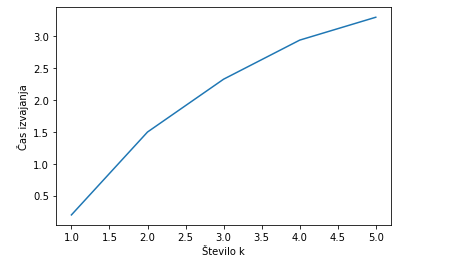
\includegraphics[width= 0.8\textwidth]{cas_od_k}
  \caption{naslov slike}
\end{figure}

\subsection{Optimalna vrednost R}






\section{Viri}

\begin{itemize}
\item Rana, R., Garg, D. (2011). An Evaluation of K-Center Problem Solving Techniques,towards Optimality. Dostopno na: https://www.longdom.org/open-access/an-evaluation-of-kcenter-problem-solving-techniques-towards-optimality-0976-4860-2-206-214.pdf?fbclid=IwAR2KDCBmif7PnRmwStiAYKnHX4Gw6UFae0h4sAo-UPN7rUaT7uRH1Ys8unc

\end{itemize}





\end{document}
